\chapter{自己結合とSELECT}

\section{自己結合}

データベースのテーブル間の結合には、自己結合というものがあります。
これは、どのような概念なのでしょうか。

自己結合というのはその名のとおり、あるテーブルが、自分自身を結合の相手として、JOINすることです。
レコードを含んだテーブルが存在するとします。このテーブルを仮にmiscという名前としましょう。

次に、miscテーブルと、同じ構造と同じレコードを含んだテーブルが存在すると仮定します。この、たまたま同じ構造とレコードを持つのテーブルを、misc\_aという名前にしましょう。

JOINの場合、同じ名前のテーブル、つまり同じテーブルをそのまま結合することはできません。
そこで、AS句をつかって、エイリアスで名前の違うテーブルが結合しているよう記述します。

\section{自己結合の内部結合と左右結合}

同じ構造とレコードを持つテーブル同士を内部結合することについて、まず考えましょう。結合してできる集合のレコードの数は、元のレコード数の2乗と同じか、それよりも小さくなります。これは、レコード同士が結合するかについて、条件判定が入るためです。

左右結合、もしくは内部結合による自己結合は、どのような場合に使うのでしょうか。それは、テーブルの中のレコード同士の比較を行って、その結果を得たい場合です。

SELECTでは、そのままでは同じテーブルの中のレコードの比較を行うことはできません。そのため、自己結合で、比較結果が真となるレコードが結合するようにします。
たとえば、数値が入ったフィールドの値で、大小を比較することにしましょう。結合条件をクエリ\ref{sql:inner}のように書けば、結合もとのレコードに対して、それよりも比較対象のフィールドの値が小さいレコードが結合したレコードを得ることができます。

\begin{lstlisting}[caption=自己結合の内部結合,label=sql:inner]
anytable AS t1 INNER JOIN anytable AS t2 
ON t1.anyfield > t2.anyfield
\end{lstlisting}

\subsection{特定のレコードより小さいレコードを取り出す}

内部結合を使う例として、特定のレコードより小さいレコードを取り出す問題を考えます。以下のようなuserテーブルが定義されているとします。

\begin{lstlisting}[caption=usersテーブル定義,label=sql:createusers]
CREATE TABLE users (id int , score int);
INSERT INTO users VALUES
  (1,100),(2,300),(3,10),(4,5),(5,70);
\end{lstlisting}

このテーブルusersを一覧すると、表\ref{table:users}のようになります。

\begin{table}[htbp]
  \begin{tabular}{|r|r|} \hline
    id & score \\ \hline \hline  
    1 & 100 \\
    2 & 300 \\
    3 & 10 \\
    4 & 5 \\
    5 & 70 \\ \hline
  \end{tabular}
  \caption{usersテーブル}
  \label{table:users}
\end{table}


ここで、idが1のレコードのscoreよりも、scoreが小さいレコードを取り出します。そのために、内部結合を利用して、クエリ\ref{sql:inner1}のように記述します。

\begin{lstlisting}[caption=特定のレコードのscoreよりもscoreがが小さいレコードw探す,label=sql:inner1]
SELECT t1.id , t2.score , t2.id , t2.score
  FROM users AS t1 LEFT JOIN users AS t2
    ON t1.score > t2.score
  WHERE t1.id=1
;
\end{lstlisting}

クエリ\ref{sql:inner1}を実行すると、表\ref{table:usersres}のような実行結果が得られます。ここでは一覧を見やすくするために結合元の情報を残していますが、この例でエイリアスt2のテーブルのフィールドだけ取り出すこともできます。


\begin{table}[htbp]
  \begin{tabular}{|r|r|r|r|} \hline
    id & score & id & score \\ \hline \hline  
    1 & 100 & 3 & 10 \\
    1 & 100 & 4 & 5 \\
    1 & 100 & 5 & 70 \\ \hline
  \end{tabular}
  \caption{id=1のscoreよりscoreが小さいレコード}
  \label{table:usersres}
\end{table}

\subsection{あるレコードが、何番目なのかの番号付けをする}

内部結合を使うもう一つの例として、あるテーブルの中のレコードが、特定のフィールドに定義した順場で並べたとき何番目になるか、を求めます。
先ほどと同様に、ユーザごとのスコアを格納したテーブルがあったとします。

テーブルusersに、ユーザIDとスコアが格納されているとします。
このテーブルは、クエリ\ref{sql:users}で定義したusersテーブルをもう一度使います。

次の例として、テーブルusersの中で、あるレコードのスコアが上から何番目かを、SELECTだけで求めます。
その方法として、あるレコードに注目して、それと同じスコアか、それよりスコアが大きいものがいくつあるかを数ええrば、その数が順番になります。

そこで、内部結合で、結合もとのすべてのレコードが、それと同じ大きさか、それより大きいレコードと結合した集合を作ります。
その結果を、結合元テーブルのidでグループ化して、集合関数count()でレコードの数を数えれば、上から数えたときに何番目か、という順番を得ることができます。

これをクエリにすると、クエリ\ref{sql:rank}となります。

\begin{lstlisting}[caption=スコアの順位を求める,label=sql:rank]
SELECT t1.id , t1.score , count(*) AS rank
  FROM users AS t1 INNER JOIN users AS t2
    ON t1.score <= t2.score
  GROUP BY t1.id
;
\end{lstlisting}


クエリ\ref{sql:rank}を実行すると、表\ref{table:rank}のように、スコアの順番がrankとして得られます。

\begin{table}[htbp]
  \begin{tabular}{|r|r|r|} \hline
    id & score & rank \\ \hline \hline  
    1 & 100 & 2 \\
    2 & 100 & 1 \\
    3 & 100 & 4 \\ 
    4 & 5 & 5 \\
    5 & 70 & 3 \\\hline
  \end{tabular}
  \caption{スコアの順序}
  \label{table:rank}
\end{table}



\section{自己結合の外部結合}
同じ構造とレコードを持つテーブル同士を外部結合した場合、それによって得られる集合は、二つの集合を掛け合わせた直積集合です。

自己結合の対象となるテーブルの例として、表\ref{table:misc}のような、レコードが三つのテーブルを考えます。

\begin{table}[htbp]
  \begin{tabular}{|r|} \hline
    num \\ \hline \hline  
    1 \\
    2 \\
    3 \\ \hline
  \end{tabular}
  \caption{miscテーブル}
  \label{table:misc}
\end{table}





\subsection{外部結合の意味}
自己結合で外部結合するということには、組み合わせにおけるすべての可能性を網羅する、という意味があります。
言葉を変えると、テーブルのフィールドを座標軸とした多次元の空間を作る、ということでもあります。



このテーブルを、自己結合で外部結合すると、表\ref{table:miscouter}ように、すべてのレコードの組み合わせを網羅した集合が得られます。
実際のSQLでは、AS句でテーブル名にエイリアスを設定して、同じ構造とレコードの別のテーブルがあるように見せると説明しました。

たとえば、外部結合した集合のレコードをすべて表示するとき、クエリ\ref{sql:outer}のようなSELECTを書きます。外部結合の結合相手として、結合元の別名を持ってきます。これは、SQLでは、同じ名前のテーブルをそのまま結合することができないためです。

\begin{lstlisting}[caption=自己結合の外部結合,label=sql:outer]
SELECT * FROM misc , misc AS misc_a;
\end{lstlisting}

クエリ\ref{sql:outer}の実行結果は、表\ref{table:miscouter}になります。フィールド名は、エイリアスをつけていないので同一のものが現れます。

\begin{table}[htbp]
  \begin{tabular}{|r|r|} \hline
    num & num \\ \hline \hline  
    1 & 1 \\
    2 & 1 \\
    3 & 1 \\ 
    1 & 2 \\
    2 & 2 \\
    3 & 2 \\
    1 & 3 \\
    2 & 3 \\
    3 & 3 \\ \hline
  \end{tabular}
  \caption{miscテーブルの自己外部結合}
  \label{table:miscouter}
\end{table}


後者は一見違うことのようですが、入力する空間を決める、ということは、とりうる値を網羅するということでもあります。

簡単な例でいくと、先ほどあげた、フィールドnumに1と2と3という値が入った、3個のレコードを持っているテーブルmiscを考えて見ましょう。

miscが座標軸の上でとりうる値であると考えます。そうすれば、misc\_aは、miscと直交するもうひとつの座標軸と考えることができます。この座標軸は、それぞれ、整数で1から3の場所が定義されています。

そのため、この二つのテーブルの外部結合は、1から3の整数がきざまれた、直交する座標で定義される空間と考えることだできます。そして、外部結合した結果は、miscとmisc\_aによって定義された空間で、とることだできる値の網羅である、と考えることができます。

\subsection{内部結合と外部結合の関係}

自己結合で、内部結合は外部結合の部分空間と考えることができます。
これは、外部結合が組み合わせのすべての可能性を網羅するのに対して、内部結合が、結合時に条件を与えて、結合結果のレコードを選択しているからです。

内部結合が外部結合の部分空間であるという例として、クエリ\ref{sql:rank}のスコアから順位を出すSELECT文を、外部結合を使った場合に書き換えてみます。

\begin{lstlisting}[caption=外部結合で書く,label=sql:outerrank]
SELECT t1.id , t1.score , count(*) AS rank
  FROM users AS t1 , users AS t2
  WHERE t1.score <= t2.score
  GROUP BY t1.id
;
\end{lstlisting}

クエリ\ref{sql:outerrank}は、内部結合を用いたクエリ\ref{sql:rank}で、ON句で書いた結合条件は、WHEREでレコードを選択する条件となります。それで選択されたレコードすべてが、グルーピングの対象となります。

その結果、内部結合を使用した場合と、おなじ結果の出力が得られます。ですが、入力側の集合が異なることと、WHERE句の有無の違いと、一見すると、命題が異なっています。

ですが、元の空間が自己結合前のテーブルであると見たとき、すべての可能性から、SELECTで解へのマッピングを行うことと、内部結合の条件として、入力を選択して問題を解くのは等価です。

\subsection{関数としてのSELECTで問題を解く}

SELECTは関数です。テーブルを入力として、テーブルを出力する、二つのテーブルの間をマッピングする関数であるという説明は、前著の「ゆるいSQL]で何度も行いました。

これは、すべての可能性という空間から、解答が存在する空間へのマッピングとして定義できる問題であれば、SELECT文で解くことができるということです。
本書では、その例として、三平方の定理と、4-Queenを1文のSELECTで解く方法について説明します

\subsection{SELECTでの問題解決の問題}

本書では、自己結合を利用する例として取り上げていますが、SQLで三平方の定理や4-Queenといった問題を解くのは、あまりよい方法とはいえません。以降で紹介するのは、いささか技芸に走ったものでもあります。

理由として、有限の個数のレコードで、入力の範囲を定義したテーブルを作成しておく必要があるためにです。
そのため、1から100の整数の範囲、という場合は100個のレコードが必要となります。
また、そのような性質から、実数の範囲など、有限のレコード数で表せないものを入力とすることもできません。

このような問題を解く場合は、入力を遅延評価で自動生成することができるHaskelなど、より実用的に行うことができる言語を利用すべきでしょう。

また、本書では取り上げていませんが、過程を求める問題も、SELECTだけで解くことはできません。SQLで処理することは不可能ではありませんが、すべての可能性としての入力を、関数としてのSELECTで解答にマッピングする、という方法では取り扱うことができません。

このような問題の例として、ライフゲームやハノイの塔の問題があります。

\subsection{三平方の定理}

三平方の定理は、直角三角形の長辺の二乗と、残りの短辺をそれぞれを2乗した者を足したものが等しいという、誰でも知っている法則です。

この、三平方の定理を、SELECTを利用して解くことができるか考えてみます。
数学的には、実数集合から、解に該当するリストの集合へのマッピング、となります。

ただし、SELECTで解く場合、元の空間もテーブルとして書ける、有限のものである必要があります。
ここでは、フィールドlengthに1から10までの整数がはいったテーブル、numsを、クエリ\ref{sql:int}のように定義します。

\begin{lstlisting}[caption=整数テーブル,label=sql:int]
CREATE TABLE nums (length int);
INSERT INTO nums VALUES
   (1),(2),..(中略)..,(9),(10);
\end{lstlisting}

このテーブル、numsに格納された整数の中で、三平方の定理が成立する組み合わせを探す、というように、問題を限定します。

\begin{lstlisting}[caption=三平方の定理の解,label=sql:square]
SELECT DISTINCT t1.length,t2.length,t3.lengh 
  FROM nums AS t1, nums AS t2, nums AS t3
  WHERE pow(t1.length,2) = 
    pow(t2.length,2) + pow(t3.length,2) 
;
\end{lstlisting}

\begin{figure}[htbp]
  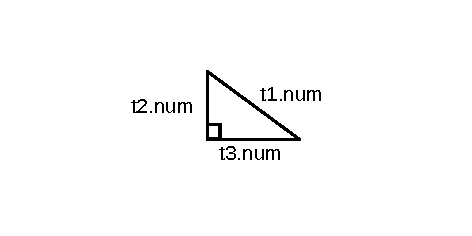
\includegraphics[width=8cm,pagebox=cropbox]{draw/fig1.pdf}
  \caption{直角三角形の辺とエイリアスの対応}
  \label{fig:triangle}
\end{figure}

クエリ\ref{sl:square}を実行すると、numsに別名を付けてつくったテーブルt1とt2とt3の直積から、三平方の定理を満たすt1.lengthとt2.lengthとt3.lengthの組み合わせをフィールドにもつテーブルが、解として出力されます。

エイリアスと直角三角形の辺の対応関係は、図\ref{fig:triangle}のように、長辺をt1、短辺をt2とt3としています。

クエリ\ref{sql:square}を実行した結果は、表\ref{table:square}のように得られます。10以下の整数で三平方の定理が成立する組み合わせのすべてが得られていることがわかります。

\begin{table}[htbp]
  \begin{tabular}{|r|r|r|} \hline
    length & length & length \\ \hline \hline  
    5 & 4 & 3 \\
    5 & 3 & 4 \\
    10 & 8 & 6 \\
    10 & 6 & 8 \\ \hline
  \end{tabular}
  \caption{三平方の定理の解}
  \label{table:square}
\end{table}


ただし、このWHERE以降の条件は三平方の定理のみに注目したものです。長辺を底辺にした場合の、軸対称の三角形の解のペアは排除されません。


\subsection{4 Queen}

n-Queenという問題があります。これは、縦横nマスの盤面で、チェスのクイーンをn個配置する問題です。このクイーンを配置する条件は、全てのクイーンがお互いを取れないことです。
チェスのルールでは、クイーンは縦横斜めにどこまでも移動できます。つまり、n個のクイーンが、お互いに縦横斜め全て重ならないように置く問題となります。

たとえば、二つのクイーンを盤面でお互いが取り合わないように配置すると、図\ref{fig:n-queen}のようになります。

\begin{figure}[htbp]
  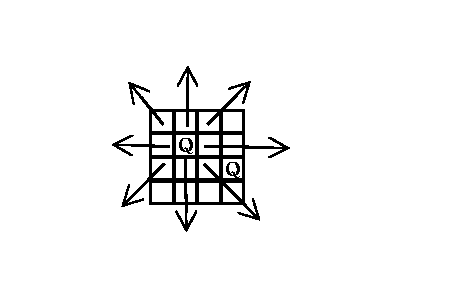
\includegraphics[width=8cm,pagebox=cropbox]{draw/4queen-0.pdf}
  \caption{n-queen問題}
  \label{fig:n-queen}
\end{figure}


n-Queenは、nが4より大きいときに解ができます。再帰の利用例として、総当たり探索で解く問を題として紹介されることが多いものです。

ここでは、n-Queenの最小問題である、4-QueenをSELECTで解いてみます。

\subsubsection{4-Queen問題をモデリングする}

まず、4-Queenの問題を、SELECTで扱えるようにしましょう。n-Queenの解は、かならず縦の1列に、ひとつだけ入ります。これは、同じ縦の列に、二つ以上のクイーンが入ることはない、という性質からです。

この性質を利用して、縦の1列列を現すテーブルcolを、クエリ\ref{sql:col}のように定義します。

\begin{lstlisting}[caption=縦の列を定義するテーブル,label=sql:col]
CRETE TABLE col (pos int);
INSERT INTO col VALUES
   (1),(2),(3),(4);
\end{lstlisting}

ある縦の列でQueenをどこに置くかは、colテーブルからどのレコードを選択したかで現します。レコードと縦の位置の対応は、図\ref{fig:column}のようになります。

\begin{figure}[htbp]
  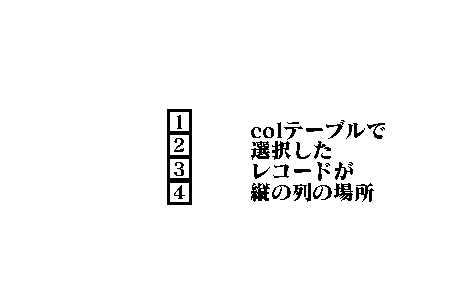
\includegraphics[width=8cm,pagebox=cropbox]{draw/4queen-1.pdf}
  \caption{盤面の縦の列のモデリング}
  \label{fig:column}
\end{figure}


4-Queenの盤面は、colテーブル4個の外部結合として現されます。このとき、4-Queenの解は、4の4乗で256のレコードを持つ、直積集合、つまり外部結合で作られたテーブルから、4-Queenの解に合致するものを選択する、という問題にすることができます。

\begin{figure}[htbp]
  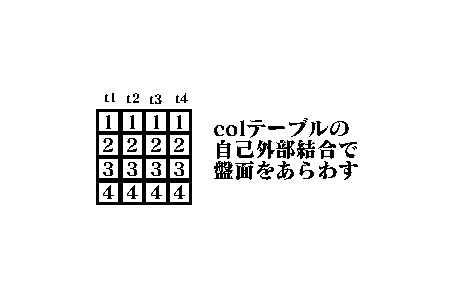
\includegraphics[width=8cm,pagebox=cropbox]{draw/4queen-2.pdf}
  \caption{外部結合で盤面をモデリングする}
  \label{fig:board}
\end{figure}

\subsubsection{問題を解く}

4-Queenを解くめには、ある縦の列のQueenに注目したとき、横や斜めの位置にくるQueenがない、という条件が全ての列に対して成立するレコードを、直積から選択するクエリを書けばよいということになります。

テーブルcolにt1からt4の、4つのエイリアスをつけ、縦の列をあらわします。それを外部結合して、盤面をあらわします

WHERE句の条件として、あるテーブルのレコードと同じ値のレコードは、ほかのテーブルでは選択しないようににします。これで、横にならぶQueenがない、という条件を判定します。

次に、あるテーブルのレコードで表される位置を選択したとき、ほかのテーブルで、斜めにあたる位置にQueenを置かない、という条件を入れます。たとえば、一番左の位置に相当するt1の任意のレコードを選択したとき、t2でそのレコードより1大きいレコード、t3でそのレコードより2大きいレコード、t4でそのレコードより3大きいレコードを排除します。

\begin{lstlisting}[caption=4-Queenを解く,label=sql:4queen]
SELECT t1.pos,t2.pos,t3.pos,t4.pos
  FROM col AS t1,col AS t2,col AS t3,col AS t4
  WHERE 
  # 1列目の横と斜め方向を排除
      t1.pos != t2.pos AND t1.pos = t3.pos AND t1.pos=t4.pos
  AND t1.pos+1 != t2.pos AND t1.pos+2 != t3.pos 
  AND t1.pos+3 != t4.pos
  # 2列目の横と斜め方向を排除
  AND t2.pos != t3.pos AND t2.pos != t4.pos
  AND t2.pos+1 != t1.pos AND t2.pos+1 != t3.pos
  AND t2.pos+2 != t4.pos
  # 3列目の横と斜め方向の排除
  AND t3.pos != t4.pos
  AND t3.pos+2 != t1.pos AND t3.pos+1 != t2.pos
  AND t3.pos+1 != t4.pos
  # 4列目の斜め方向の排除
  AND t4.pos+3 != t1.pos AND t4.pos+2 != t4.pos
  AND t4.pos+1 != t3.pos
;
\end{lstlisting}

クエリ\ref{sql:4queen}は、鏡面対称の解は排除しません。また、縦方向はかならずひとつしかクイーンが入らない、という、向きの制限をしたモデリングを行っているので、回転対称の解は得られません。

クエリ\ref{sql:4queen}で、クイーンの配置は、表\ref{table:4queen}のように得られます。


\begin{table}[htbp]
  \begin{tabular}{|r|r|r|r|} \hline
    pos & pos & pos & pos \\ \hline \hline  
    3 & 1 & 4 & 2 \\
    2 & 4 & 1 & 3 \\ \hline
  \end{tabular}
  \caption{4-Queenの解}
  \label{table:4queen}
\end{table}

表\ref{table:4queen}の結果にしたがって、図\ref{fig:result}のように、盤面にクイーンを配置ぢます。
そうすると、4-Queen問題がSELECT文で解けたことがわかります。



\begin{figure}[htbp]
  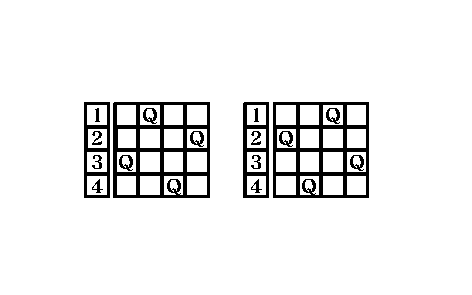
\includegraphics[width=8cm,pagebox=cropbox]{draw/4queen-3.pdf}
  \caption{4-Queenの解}
  \label{fig:result}
\end{figure}
